\subsection{\textit{Semantic Web Service Offer Discovery for E-Commerce} \cite{kopecky2008semantic}} \label{sec:sws-offer}

A Web Semântica é uma extensão da atual Web com descrições semânticas de dados e serviços que podem ser usados automaticamente por um computador em nome de seu usuário \cite{kopecky2008semantic}. Para tornar os \textit{Web Services} parte da Web Semântica, a área de pesquisa de Web Services Semânticos (\textit{Semantic Web Services}, SWS\nomenclature{SWS}{\textit{Semantic Web Services}}) tem como objetivo, aumentar o nível de automação ao redor dos \textit{Web Services}. Automação de SWS é suportada por descrições semânticas processáveis por computador, que captura aspectos importantes do significado de operações e mensagens de serviços. \cite{kopecky2008semantic}

A automação dos Web Services é realizada em um \textit{Semantic Execution Environment} (SEE\nomenclature{SEE}{\textit{Semantic Execution Environment}}). Este ambiente é responsável por receber um objetivo concreto de um usuário e cumprí-lo, localizando e usando apropriados WSs disponíveis, como apresentado na Figura \ref{fig:SEE}.

\begin{center}
	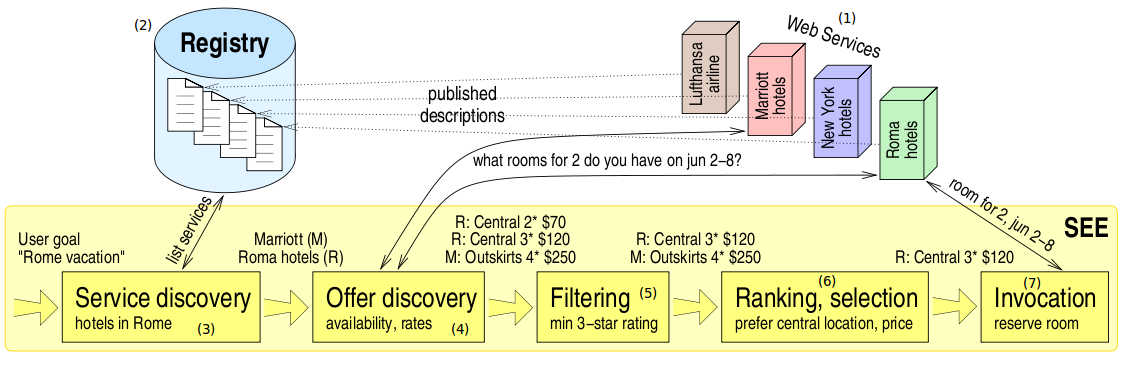
\includegraphics[width=1\textwidth]{images/see.png}
	\captionof{figure}{Automação de tarefas em um \textit{Semantic Execution Environment} (adaptada de \cite{kopecky2008semantic}).}
	\label{fig:SEE}
\end{center}

Na Figura \ref{fig:SEE}, existem alguns serviços registrados (1) em um repositório (2). O usuário deseja uma vaga em um hotel em Roma (3), então o SEE busca uma lista de serviços registrados de hotéis em Roma. Continuando, o SEE descobre ofertas\footnote{O termo "descoberta de ofertas" é cunhado pelos autores em \cite{kopecky2008semantic} como um sinônimo de "descoberta de serviços", apenas para fazer distinção entre o \textit{Web Service} em si e os serviços disponibilizados por ele (as operações).}, baseado em preços e disponibilidade de quartos, interagindo com os serviços encontrados (4). Em seguida o SEE, baseado nos critérios do usuário, filtra os resultados para que sejam obtidos apenas os hotéis que tenham classificação mínima de três estrelas (5) e classifica-os, selecionando aquele que tenha o menor preço e esteja no centro da cidade (6). Após a seleção, é feita a invocação do serviço para reserva de um quarto (7).

Existem alguns \textit{frameworks} de SWS que suportam automação, como esboçado na Figura \ref{fig:SEE}; os maiores são o \textit{Web Service Modeling Ontology} (WSMO)\footnote{\url{http://www.wsmo.org}}\nomenclature{WSMO}{\textit{Web Service Modeling Ontology}} e o \textit{Semantic Markup for Web Services} (OWL-S)\footnote{\url{http://www.w3.org/Submission/OWL-S}, no entanto, nenhum deles suporta a descoberta de oferta. Desta forma, o trabalho apresentado em  \cite{kopecky2008semantic} propõe o WSMO-Lite, um \textit{framework} leve para SWS, que adiciona anotações semânticas à descrição de Web Service.

\subsubsection{Descoberta de Oferta de Serviço}

O objetivo da descoberta de oferta de serviço é descobrir, classificar e selecionar serviços. A descoberta retorna um conjunto de serviços que podem potencialmente atingir o objetivo do usuário.  A descoberta de oferta é a interação com estes serviços (ou provedores de serviços), que resulta em um conjunto de ofertas, de onde deve-se selecionar alguma oferta relevante para o usuário. Este conjunto é então filtrado e classificado, de acordo com critérios do usuário, para permitir a seleção do melhor serviço. Por último, o serviço selecionado é consumido. \cite{kopecky2008semantic}

\subsubsection{Anotações Semânticas em WS com WSMO-\textit{Lite}}

Descoberta de oferta semântica pode, opcionalmente, ser capaz de realizar comunicação com qualquer WS que proveja operações para busca de informações sobre seus serviços. Para conseguir isto, o motor de descoberta de oferta precisa de uma descrição da interface do serviço, para ver quais operações o serviço contém, que podem ser usadas para obter informações de ofertas; e uma descrição dos dados trocados, para entender as ofertas e ser capaz de compará-las com o objetivo do usuário. \cite{kopecky2008semantic}

Qualquer serviço, descrito em WSDL, tem uma interface que consiste de operações. O WSMO-\textit{Lite} anota a interface e operações do \textit{Web Service} com semânticas funcionais, e os parâmetros de entrada e saída das operações são anotados com semânticas de informação.

O \textit{framework} utiliza a semântica de operações seguras do WSDL 2.0\footnote{Segundo a W3C\cite{w3c-wsdl-safety}, uma interação segura é aquela em que o cliente não tem nenhuma obrigação ao utilizar um determinado serviço, não estando obrigado a realizar nenhum contrato com o provedor. Por exemplo, ao acessar um método para consulta de preços de quartos em um hotel, o cliente não está obrigado a realizar a reserva. Métodos seguros são definidos no WSDL com o uso do atributo \textit{safe}.} para obter uma lista de métodos que fornecem informações sobre serviços disponibilizados (como métodos para obtenção de classificação de estrelas de um hotel, valores das reservas, disponibilidade, etc.

\subsubsection{Conclusões}

A proposta apresentada em \cite{kopecky2008semantic} implementa um \textit{framework} denominado WSMO-\textit{Lite}, para incluir anotações semânticas leves em arquivos WSDL, para permitir a automatização de descoberta de ofertas. O \textit{framework} é baseado em um \textit{Semantic Execution Environment} que permite que um usuário encontre ofertas de serviços, baseado em objetivos por ele definidos. A arquitetura apresentada é bastante interessante pois permite não somente a descoberta de serviços, mas a automatização da realização dos objetivos do usuário, como reservar um quarto de hotel, baseado em critérios como total de estrelas do hotel, preço e localização, sem que o usuário precise acessar cada um dos serviços disponibilizados para ele mesmo decidir qual o melhor.
